\documentclass{article}

\usepackage{graphicx}
\usepackage{tikz}
\usepackage{tikzsymbols}
\usetikzlibrary{calc,patterns,shapes.geometric}
\pagestyle{empty}
\usepackage[margin=0pt]{geometry}
\geometry{papersize={14in,12in}}

\def\centerarc[#1](#2)(#3:#4:#5){\draw[#1] ($(#2)+({#5*cos(#3)},{#5*sin(#3)})$) arc (#3:#4:#5);}

\begin{document}
	\begin{figure}
		\centering
		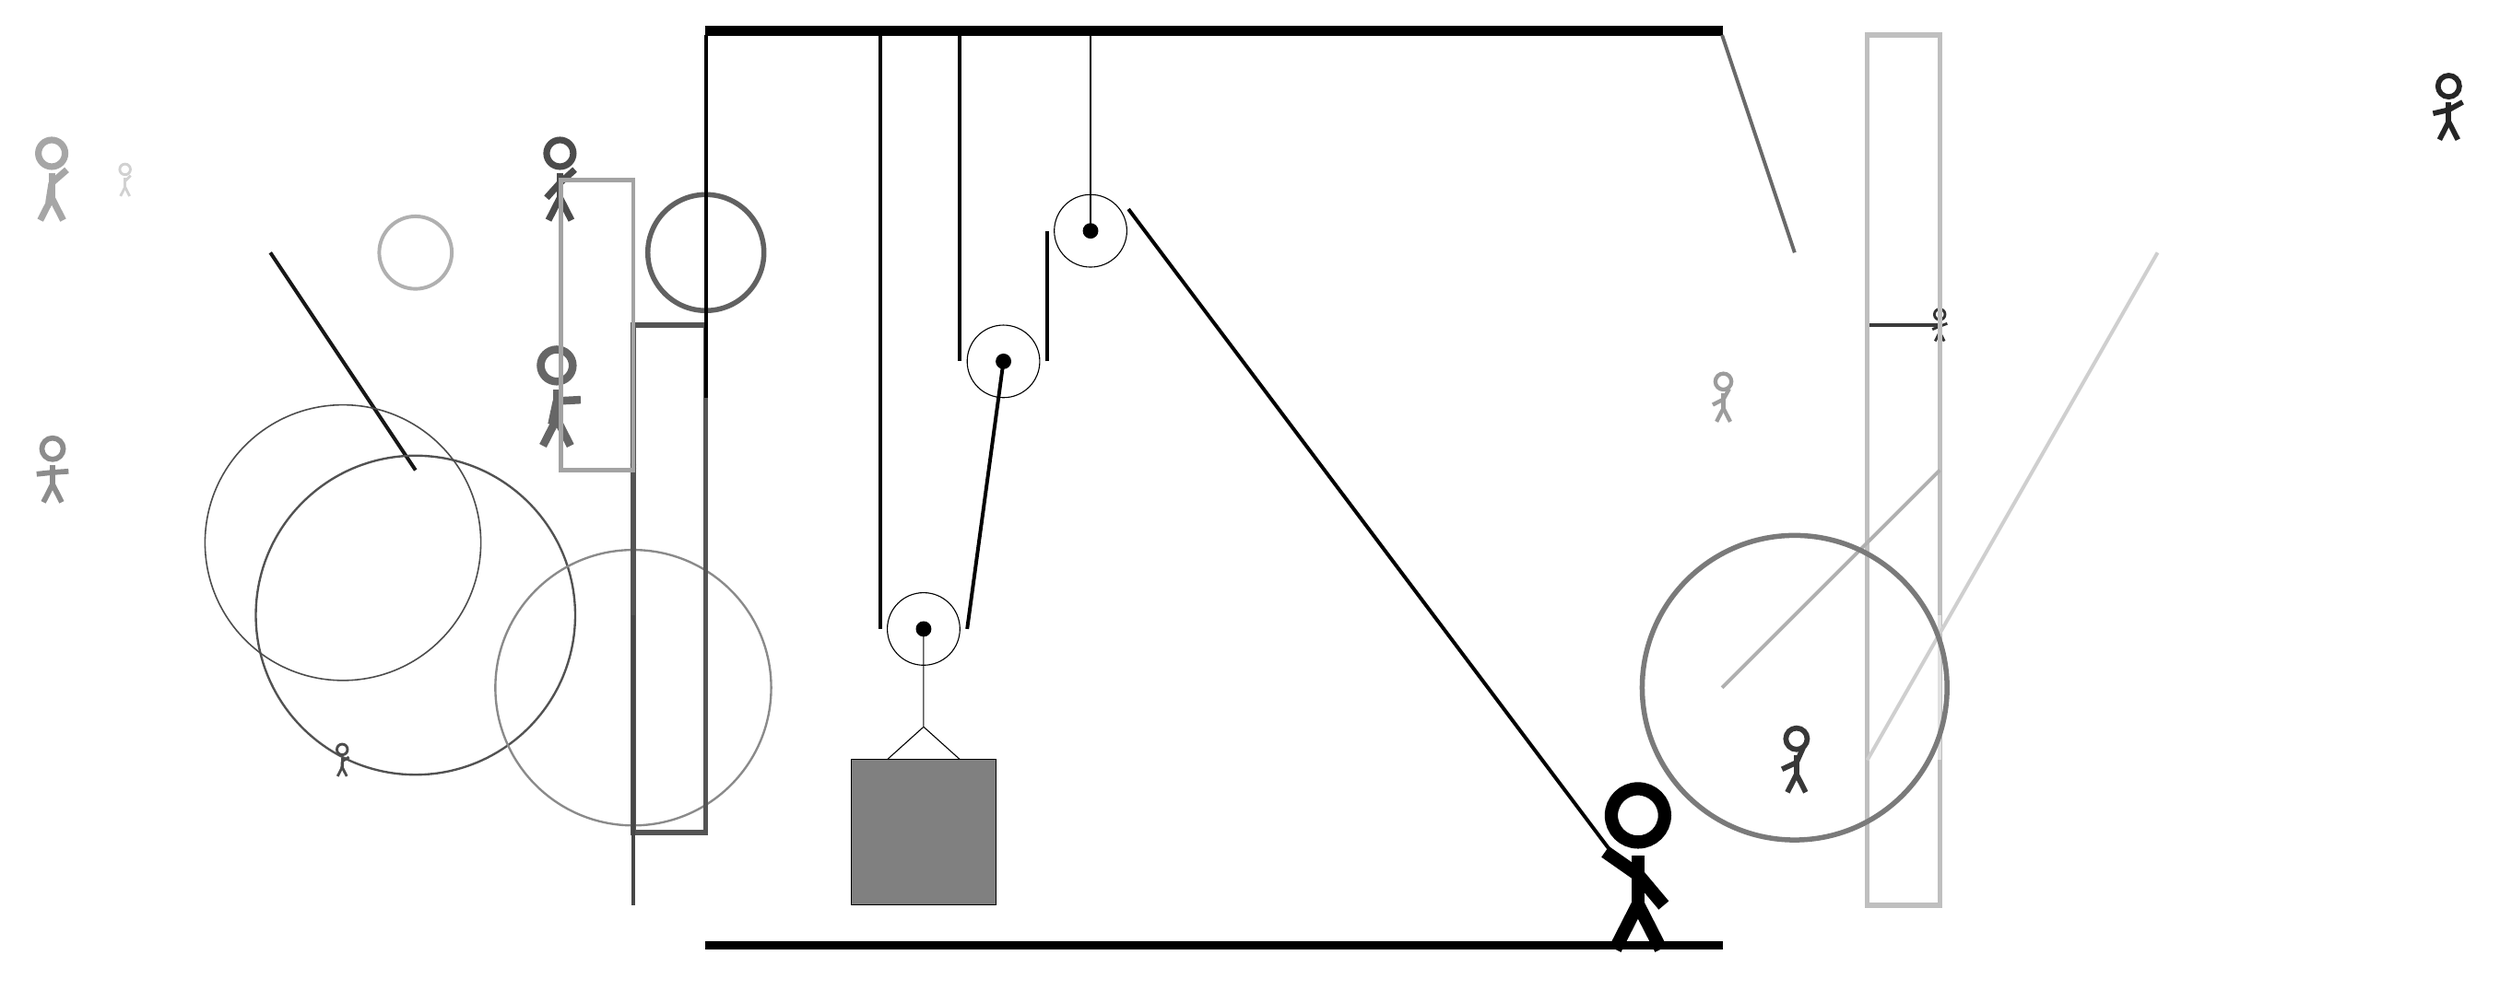
\begin{tikzpicture}
			%%%%% START %%%%%
			
			\draw[fill=black] (-2, 9) rectangle (12, 9.125);
			
			\draw (1, 0.81) circle (0.5);
			\draw[fill=black] (1, 0.81) circle (0.1);
			
			\draw (2.1, 4.5) circle (0.5);
			\draw[fill=black] (2.1, 4.5) circle (0.1);
			
			\draw[line width=0.5mm, color=black!91](-6, 3) -- (-8, 6);
			
			\draw [line width=0.7mm, color=black!62](-2, 6) circle (0.8);
			\node[line width=0.7mm, color=black!80] at (15, 5) {\Strichmaxerl[2][23][20]};
			\node[line width=0.2mm, color=black!70] at (-4, 7) {\Strichmaxerl[5][48][42]};
			
			\draw [line width=0.3mm, color=black!68](-6, 1) circle (2.2);
			\draw [line width=0.3mm, color=black!46](-3, 0) circle (1.9);
			\draw[line width=0.5mm, color=black!77] (14, 5) rectangle (15, 9);
			
			\draw[line width=0.7mm, color=black!25] (14, -3) rectangle (15, 9);
			\node[line width=0.6mm, color=black!78] at (13, -1) {\Strichmaxerl[4][25][66]};
			\draw[line width=0.5mm, color=black!12](15, 1) -- (15, -1);
			
			\node[line width=0.6mm, color=black!45] at (-11, 3) {\Strichmaxerl[4][6][4]};
			
			\node[line width=0.4mm, color=black!13] at (-3, 3) {\Strichmaxerl[1][57][41]};
			\node[line width=0.2mm, color=black!85] at (22, 8) {\Strichmaxerl[4][13][29]};
			
			\node[line width=0.5mm, color=black!18] at (-10, 7) {\Strichmaxerl[2][90][46]};
			\draw[line width=0.5mm, color=black!31](12, 0) -- (15, 3);
			\draw[line width=0.7mm, color=black!67] (-3, -2) rectangle (-2, 5);
			
			\draw[line width=0.5mm, color=black!19](14, -1) -- (18, 6);
			\node[line width=0.6mm, color=black!60] at (-4, 4) {\Strichmaxerl[6][78][3]};
			\draw [line width=0.5mm, color=black!31](-6, 6) circle (0.5);
			\node[line width=0.3mm, color=black!39] at (12, 4) {\Strichmaxerl[3][27][61]};
			\draw[line width=0.6mm, color=black!36] (-4, 7) rectangle (-3, 3);
			
			\draw[line width=0.5mm, color=black!59](13, 6) -- (12, 9);
			\draw [line width=0.2mm, color=black!70](-7, 2) circle (1.9);
			\node[line width=0.3mm, color=black!35] at (-11, 7) {\Strichmaxerl[5][81][41]};
			\draw [line width=0.7mm, color=black!52](13, 0) circle (2.1);
			\draw[line width=0.5mm, color=black!72](-3, -3) -- (-3, 1);
			\draw[line width=0.5mm, color=black!99](-2, 4) -- (-2, 9);
			\node[line width=0.5mm, color=black!70] at (-7, -1) {\Strichmaxerl[2][87][32]};
			
			\draw (3.3, 6.3) circle (0.5);
			\draw[fill=black] (3.3, 6.3) circle (0.1);
			\draw[thick] (3.3, 6.3) -- (3.3, 9);
			
			\draw (1, 0.81) -- (1, -0.54) -- (0.5, -0.99) -- (1.5, -0.99) -- (1, -0.54);
			\draw[fill=black!50] (0, -0.99) rectangle (2, -2.99);
			
			\draw[line width=0.5mm] (0.4, 9) -- (0.4, 0.81);
			\centerarc[line width=0.5mm](1, 0.81)(180:360:0.6);
			\draw[line width=0.5mm](1.6, 0.81) -- (2.1, 4.5);
			\draw[line width=0.5mm] (1.5, 9) -- (1.5, 4.5);
			\centerarc[line width=0.5mm](2.1, 4.5)(180:360:0.6);
			\draw[line width=0.5mm](2.7, 4.5) -- (2.7, 6.3);
			\centerarc[line width=0.5mm](3.3, 6.3)(30:180:0.6);
			\draw[line width=0.5mm] (3.822, 6.6) -- (10.5, -2.3);
			
			\node at (10.8, -2.5) {\Strichmaxerl[10][-35][-50]};
			
			\draw[fill=black] (-2, -3.5) rectangle (12, -3.6);
			
			%%%%% END %%%%%
		\end{tikzpicture}
	\end{figure}	
\end{document}